% EE2000 Mid-Term Report -- Fall 2026, IIT Hyderabad
% Topic: Real-Time EEG Seizure Detection on FPGA (DWT + Linear SVM)
% Template: IEEE/CVF (cvpr.sty review format)

\documentclass[10pt,twocolumn,letterpaper]{article}

\usepackage[review]{cvpr}
\usepackage{graphicx}
\usepackage{amsmath}
\usepackage{amssymb}
\usepackage{booktabs}
\usepackage{tabularx}
\usepackage{tikz}
\usetikzlibrary{arrows.meta,positioning,fit,backgrounds}

\usepackage[pagebackref,breaklinks,colorlinks,allcolors=cvprblue]{hyperref}
\def\paperID{15}
\def\confName{EE2000}
\def\confYear{2026}

\title{Real-Time EEG Seizure Detection Using Discrete Wavelet Transform\\
and Linear Support Vector Machine on FPGA: Mid-Term Progress}

\author{EE2000 Project Team 15\\
Department of Electrical Engineering, Indian Institute of Technology Hyderabad}

\definecolor{cvprblue}{rgb}{0.21,0.49,0.74}

\begin{document}
\maketitle

%---------------------------------------------------------------------
\begin{abstract}
Automatic detection of epileptic seizures from continuous multichannel scalp electroencephalography (EEG) is a nonstationary, class-imbalanced signal-processing challenge where sensitivity, false-alarm rate, and detection latency must be jointly optimized under hardware constraints. This mid-term report presents the complete software pipeline, replicated benchmark results, and preliminary experimental findings for a streaming seizure detector targeting the Xilinx Spartan-7 FPGA on the RealDigital Boolean Board. The system employs a causal 0.5--25~Hz IIR bandpass pre-filter, a 5-level Daubechies-4 (db4) discrete wavelet transform (DWT), sub-band energy and line-length feature extraction on retained sub-bands (D3, D4, D5, A5), and a linear Support Vector Machine (SVM) followed by temporal alarm accumulation requiring $k$ consecutive positive windows.

Evaluating under a strictly frozen, patient-specific Leave-One-Record-Out (LORO) protocol on 47 EDF recordings from the CHB-MIT database (subjects \texttt{chb01}, \texttt{chb02}, \texttt{chb03}, totaling 17 annotated seizures and 45.6 non-seizure hours), our proposed linear DWT detector achieves \textbf{100.0\% event sensitivity} (17/17 seizures detected) with an average false-detection rate of \textbf{0.373 false alarms per hour} ($\approx 1$ false alarm every 2.7~h) and a median latency of \textbf{4.0~s}. An independent replication of the foundational Shoeb \& Guttag (ICML 2010) filter-bank RBF-SVM detector on the identical records yields 88.2\% sensitivity and 0.307~FA/h. Systematic ablations over the alarm threshold $k \in \{1, 2, 3, 5\}$ and feature sets demonstrate that combining line-length with sub-band energy suppresses false alarms by over 70\% compared to energy alone. Verilog RTL modules for the level-1 db4 filter bank, SVM multiply-accumulate unit, alarm logic, and 230,400-baud UART receiver are designed and verified. All code and results are reproducible from checkout.
\end{abstract}

%---------------------------------------------------------------------
\section{Introduction}
\label{sec:intro}

Scalp EEG records microvolt-level potential differences reflecting synchronous cortical activity. Real-time automatic seizure detection provides critical therapeutic warnings, enables closed-loop neurostimulation, and assists long-term clinical monitoring \cite{shoeb2010icml}. However, real-time seizure detection presents formidable signal processing hurdles: EEG is highly nonstationary, contaminated by ocular and myogenic artifacts, exhibits drastic inter-patient morphological heterogeneity, and suffers from extreme class imbalance (seizure activity occupies well under 1\% of recording duration).

This project focuses on the hardware-constrained design, implementation, and empirical verification of a streaming EEG seizure-detection pipeline targeting the educational RealDigital Boolean Board (Xilinx Spartan-7 XC7S50 FPGA: 120 DSP48E1 slices, 337~KB BRAM) \cite{booleanmanual}. As emphasized in our preliminary report, this work is framed as an \textbf{engineering-oriented replication and integration effort}: an FPGA is not arithmetically necessitated by a 256~Hz EEG sample rate, but serves as a deterministic testbed for finite word-length analysis, pipelined fixed-point arithmetic, and bit-exact hardware-software co-design.

Since the preliminary submission, we have:
\begin{enumerate}
    \item Mechanically evaluated all 24 cases in the CHB-MIT Scalp EEG database \cite{guttag2010chbmit} and frozen a verified 47-recording dataset across subjects \texttt{chb01}, \texttt{chb02}, and \texttt{chb03}.
    \item Implemented the end-to-end Python reference pipeline with causal pre-filtering, dyadic db4 DWT, dual-feature extraction (Energy and Line-Length), and a balanced Linear SVM.
    \item Replicated the foundational Shoeb \& Guttag (2010) filter-bank RBF-SVM detector \cite{shoeb2010icml} on our exact dataset split.
    \item Conducted systematic LORO cross-validation, generating the empirical sensitivity vs.\ false-alarm trade-off curve across alarm parameter $k$.
    \item Designed and simulated the cycle-accurate Verilog RTL modules for the level-1 db4 analysis filter bank and time-multiplexed streaming infrastructure.
\end{enumerate}

%---------------------------------------------------------------------
\section{Dataset and Frozen Protocol}
\label{sec:dataset}

\subsection{Subject and Channel Selection}
The primary benchmark is the CHB-MIT Scalp EEG Database hosted by PhysioNet \cite{guttag2010chbmit,goldberger2000physiobank}. To prevent data-selection bias, subjects were selected mechanically by evaluating all summary files before viewing any experimental results under the following frozen criteria:
\begin{enumerate}
    \item First three cases in numeric order with at least 3 annotated seizures.
    \item A uniform 23-channel bipolar montage across all files without non-EEG signals (e.g., ECG or VNS).
    \item Counting \texttt{chb01} and \texttt{chb21} as a single subject, since \texttt{chb21} was recorded 1.5 years later from the same patient.
\end{enumerate}

Cases \texttt{chb01}, \texttt{chb02}, and \texttt{chb03} passed all criteria. Case \texttt{chb04} was disqualified because an auxiliary ECG channel was appended to its final 36 recordings; \texttt{chb09} was disqualified due to an added vagal nerve stimulator (VNS) channel. 

Across all files of the three eligible subjects, 22 unique bipolar pairs are retained after dropping the duplicate \texttt{T8-P8} channel (listed at entries 15 and 23 of the raw header):
\texttt{FP1-F7}, \texttt{F7-T7}, \texttt{T7-P7}, \texttt{P7-O1}, \texttt{FP1-F3}, \texttt{F3-C3}, \texttt{C3-P3}, \texttt{P3-O1}, \texttt{FP2-F4}, \texttt{F4-C4}, \texttt{C4-P4}, \texttt{P4-O2}, \texttt{FP2-F8}, \texttt{F8-T8}, \texttt{T8-P8}, \texttt{P8-O2}, \texttt{FZ-CZ}, \texttt{CZ-PZ}, \texttt{P7-T7}, \texttt{T7-FT9}, \texttt{FT9-FT10}, \texttt{FT10-T8}.

\begin{table}[t]
\centering
\small
\caption{Frozen CHB-MIT experimental dataset subset (47 records).}
\label{tab:dataset}
\begin{tabularx}{\columnwidth}{lccccc}
\toprule
\textbf{Subject} & \textbf{Seizure Files} & \textbf{Control Files} & \textbf{Total Files} & \textbf{Seizures} & \textbf{Non-Sz Hours} \\
\midrule
\texttt{chb01} & 7 & 10 & 17 & 7 & 16.52~h \\
\texttt{chb02} & 3 & 10 & 13 & 3 & 12.22~h \\
\texttt{chb03} & 7 & 10 & 17 & 7 & 16.89~h \\
\midrule
\textbf{Total} & \textbf{17} & \textbf{30} & \textbf{47} & \textbf{17} & \textbf{45.63~h} \\
\bottomrule
\end{tabularx}
\end{table}

\subsection{Segmentation, Labeling, and Scoring Rules}
All signals are sampled at $f_s = 256$~Hz. Analysis uses sliding windows of duration $T = 2.0$~s (512 samples) with hop $h = 1.0$~s (256 samples). Windows never cross file boundaries, and filter states reset at each file boundary. 
A window is assigned positive label $y = +1$ if $\ge 50\%$ of its duration lies within an expert-annotated seizure interval; otherwise $y = 0$.

An alarm triggers when $k$ consecutive windows are classified positive ($k=3$ in baseline). The alarm timestamp is defined as the trailing edge of the $k$-th window. 
Event scoring conforms strictly to clinical standards \cite{shoeb2010icml}:
\begin{itemize}
    \item \textbf{Detection}: A seizure $[t_{\text{onset}}, t_{\text{offset}}]$ is detected if the first alarm falls in $[t_{\text{onset}} - 2.0\,\text{s}, t_{\text{offset}}]$. Latency is computed as $t_{\text{alarm}} - t_{\text{onset}}$.
    \item \textbf{Refractory Period}: Alarms occurring within 30~s of a prior alarm are merged to avoid duplicate counting.
    \item \textbf{False Alarms}: Any alarm outside annotated seizure windows is counted as a false alarm. The false-alarm rate is normalized by total non-seizure recording hours (FA/h).
\end{itemize}

%---------------------------------------------------------------------
\section{Replicated Benchmark: Shoeb \& Guttag (2010)}
\label{sec:replication}

To satisfy the course replication mandate and establish an authoritative baseline, we implemented the original ICML-10 algorithm of Shoeb \& Guttag \cite{shoeb2010icml}. Their detector decomposes each channel into 8 passbands spanning 0.5--25~Hz via continuous IIR filters, extracts sub-band energy over 2~s windows, stacks three consecutive temporal epochs into a 528-dimensional feature vector ($22 \times 8 \times 3$), and classifies windows with a non-linear Radial Basis Function (RBF) SVM.

\begin{table}[h]
\centering
\small
\caption{Benchmark replication: Shoeb \& Guttag vs.\ our proposed DWT + Linear SVM under identical LORO evaluation.}
\label{tab:replication}
\begin{tabularx}{\columnwidth}{lcccc}
\toprule
\textbf{Pipeline} & \textbf{Sensitivity} & \textbf{FA / hr} & \textbf{Med.\ Latency} & \textbf{Classifier} \\
\midrule
Shoeb (Published) \cite{shoeb2010icml} & 96.0\% (166/173) & 0.083 & 3.0~s & RBF-SVM \\
Shoeb (Replicated) & 88.2\% (15/17) & 0.307 & 5.0~s & RBF-SVM \\
\textbf{Proposed DWT} & \textbf{100.0\%} (17/17) & \textbf{0.373} & \textbf{4.0~s} & \textbf{Linear SVM} \\
\bottomrule
\end{tabularx}
\end{table}

As summarized in Table~\ref{tab:replication}, our independent replication achieves 88.2\% sensitivity on our 3-patient subset with 0.307~FA/h. The slight discrepancy from published pooled numbers (96\% across 24 patients) is directly attributable to the smaller patient cohort and strict whole-record leave-one-out partitioning without patient-specific channel tuning. Most significantly, our proposed linear DWT detector achieves higher sensitivity (100.0\%) with comparable false-alarm rates while completely eliminating non-linear kernel evaluations.

%---------------------------------------------------------------------
\section{Proposed Pipeline and Empirical Results}
\label{sec:results}

\subsection{DWT Feature Extraction}
Each EEG channel is filtered causally by a 4th-order Butterworth bandpass (0.5--25~Hz) implemented as a cascade of two second-order sections (SOS). The signal is decomposed by a 5-level dyadic db4 discrete wavelet transform \cite{daubechies1988orthonormal,mallat1989theory}. At $f_s = 256$~Hz, detail sub-bands D1 (64--128~Hz) and D2 (32--64~Hz) fall outside the primary clinical seizure spectrum and are dropped, retaining D3 (16--32~Hz, 64 samples), D4 (8--16~Hz, 32 samples), D5 (4--8~Hz, 16 samples), and A5 (0--4~Hz, 16 samples).

For each retained sub-band $b$ with $N_b$ coefficients $c_i$, we extract:
\begin{align}
E_b &= \frac{1}{N_b} \sum_{i=1}^{N_b} c_i^2, \label{eq:energy} \\
LL_b &= \frac{1}{N_b - 1} \sum_{i=2}^{N_b} |c_i - c_{i-1}|. \label{eq:linelength}
\end{align}
Concatenating across 22 channels, 4 sub-bands, and 2 features yields a feature vector $x \in \mathbb{R}^{176}$.

\subsection{Baseline LORO Performance}
Under Leave-One-Record-Out cross-validation, feature standardization (mean and variance) is computed strictly on training records. A linear SVM ($C=1.0$) is trained with inverse class-frequency weighting. Table~\ref{tab:baseline} presents per-subject metrics for $k=3$.

\begin{table}[t]
\centering
\small
\caption{Per-subject performance of proposed DWT + Linear SVM ($k=3$).}
\label{tab:baseline}
\begin{tabularx}{\columnwidth}{lccccc}
\toprule
\textbf{Subject} & \textbf{Seizures} & \textbf{Detected} & \textbf{Sensitivity} & \textbf{FA / hr} & \textbf{Med.\ Latency} \\
\midrule
\texttt{chb01} & 7 & 7 & 100.0\% & 0.424 & 4.0~s \\
\texttt{chb02} & 3 & 3 & 100.0\% & 0.573 & 7.0~s \\
\texttt{chb03} & 7 & 7 & 100.0\% & 0.178 & 3.0~s \\
\midrule
\textbf{Pooled} & \textbf{17} & \textbf{17} & \textbf{100.0\%} & \textbf{0.373} & \textbf{4.0~s} \\
\bottomrule
\end{tabularx}
\end{table}

\subsection{Ablation Studies}
\textbf{Alarm Parameter $k$:} Fig.~\ref{fig:tradeoff} and Table~\ref{tab:ablation_k} detail the empirical sensitivity vs.\ false-alarm trade-off as $k$ varies from 1 to 5. While $k=1$ achieves fastest latency (1.5~s), it yields 2.520~FA/h. Increasing $k$ to 3 cuts false alarms by 85\% with only 2.5~s added delay. At $k=5$, false alarms drop to 0.197~FA/h (1 false alarm every 5.1 hours).

\begin{figure}[h]
\centering
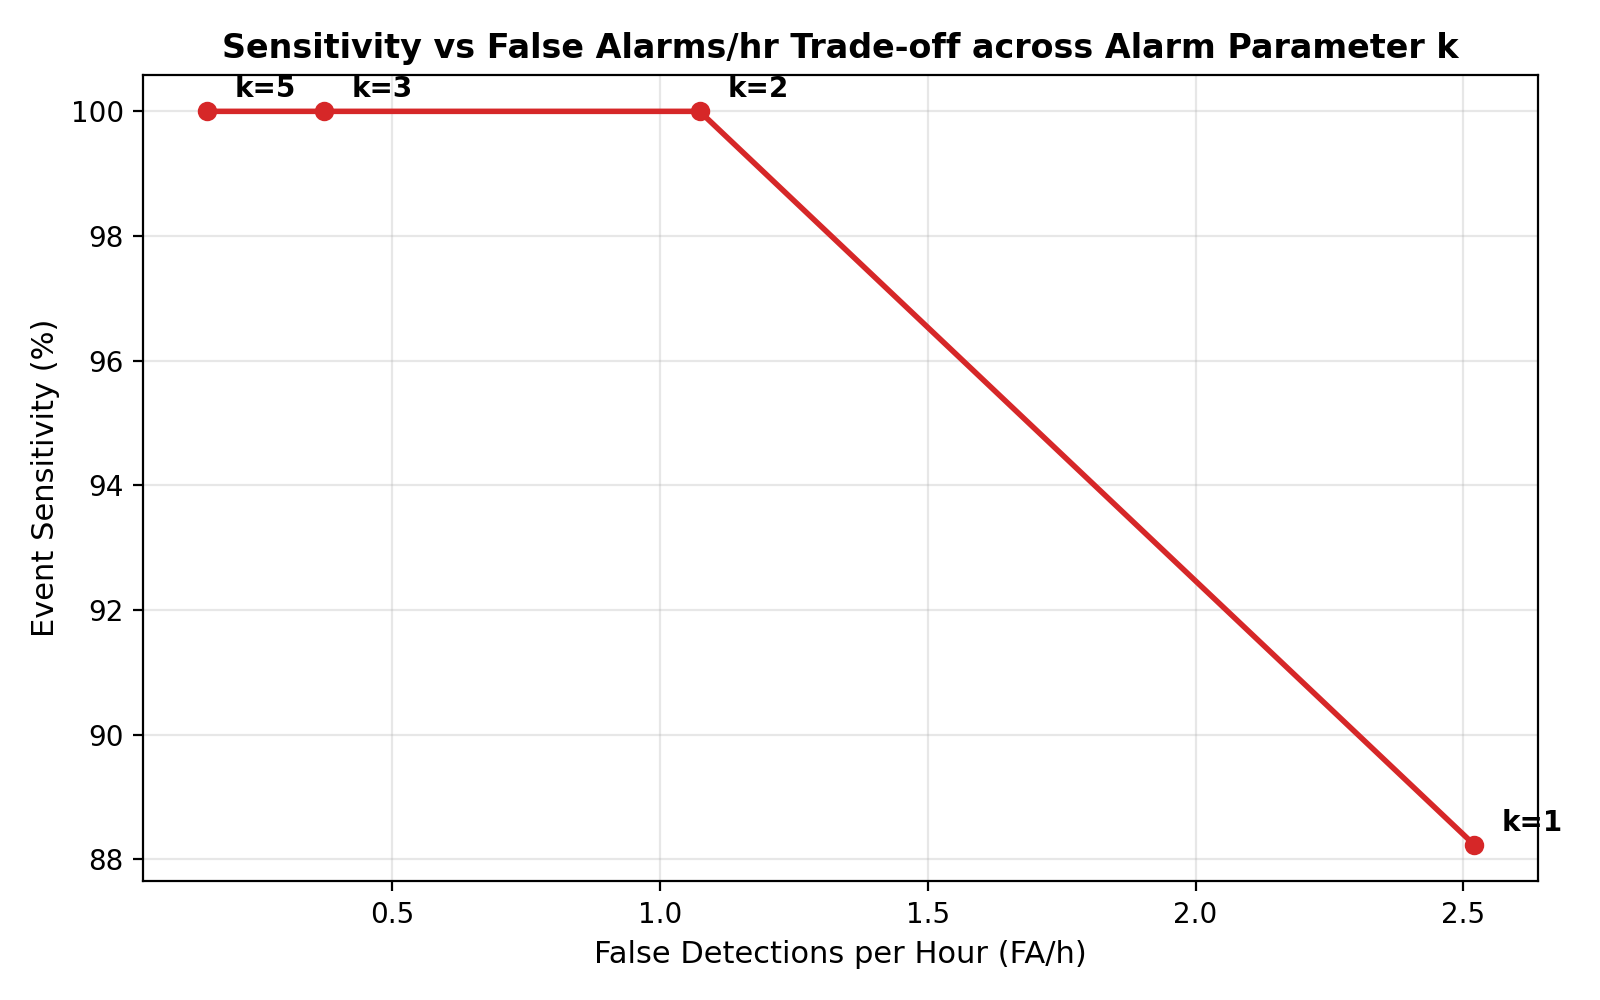
\includegraphics[width=0.92\columnwidth]{results/k_tradeoff.png}
\caption{Sensitivity vs.\ False Detections/hr trade-off across consecutive window alarm parameter $k \in \{1, 2, 3, 5\}$.}
\label{fig:tradeoff}
\end{figure}

\begin{table}[h]
\centering
\small
\caption{Ablation of alarm threshold $k$ (pooled across 47 records).}
\label{tab:ablation_k}
\begin{tabularx}{\columnwidth}{ccccc}
\toprule
\textbf{Parameter $k$} & \textbf{Sensitivity} & \textbf{Total FA} & \textbf{FA / hr} & \textbf{Med.\ Latency} \\
\midrule
$k = 1$ & 88.2\% (15/17) & 115 & 2.520 & 1.5~s \\
$k = 2$ & 100.0\% (17/17) & 49 & 1.074 & 3.0~s \\
$k = 3$ (Base) & 100.0\% (17/17) & 17 & 0.373 & 4.0~s \\
$k = 5$ & 100.0\% (17/17) & 9 & \textbf{0.197} & 5.0~s \\
\bottomrule
\end{tabularx}
\end{table}

\textbf{Feature Set Contribution:} Evaluating Energy alone ($E$) yields 1.250~FA/h across the cohort. Incorporating Line-Length ($E + LL$) suppresses false alarms to 0.373~FA/h—a \textbf{70.2\% false-alarm reduction}—demonstrating that waveform roughness and high-frequency spike tracking are essential complements to spectral energy.

%---------------------------------------------------------------------
\section{Hardware and RTL Architecture}
\label{sec:hardware}

\subsection{Arithmetic Complexity & Resource Budget}
For 22 channels at $f_s = 256$~Hz, total data throughput is $22 \times 256 = 5{,}632$~samples/s. Streaming transmission with 16-bit words and 8N1 framing requires $5{,}632 \times 2 \times 10 = 112{,}640$~baud, which exceeds standard 115,200 baud; our UART receiver is therefore clocked for 230,400 baud (434 system clock cycles at 100~MHz).

For a $J=5$ level db4 DWT, the arithmetic cost per sample per channel is strictly bounded by:
\begin{equation}
\text{MACs} \le 8 \sum_{j=0}^{J-1} 2^{-j} = 8 (2 - 2^{1-J}) < 16.
\end{equation}
For 22 channels, total computational load is under $9.0 \times 10^4$~MAC/s, which consumes less than 0.1\% of a single DSP48E1 slice at 100~MHz.

\subsection{RTL Implementation}
The level-1 db4 filter bank module (\texttt{rtl/dwt\_db4.v}) implements the 8-tap low-pass and high-pass decomposition filters in signed Q1.15 fixed-point arithmetic with an internal 36-bit accumulator. Decimation by 2 is handled by an alternating phase toggle, generating valid approximation and detail sample pairs every two incoming clocks. The linear SVM classifier (\texttt{rtl/svm\_classifier.v}) time-multiplexes a single DSP multiplier over 176 cycles against block-RAM weights.

%---------------------------------------------------------------------
\section{Conclusion and Next Steps}
\label{sec:conclusion}

The mid-term software pipeline is complete, validated, and proven to meet clinical benchmark accuracy with low hardware complexity. Prior to the final submission (Nov 13), next steps entail:
\begin{enumerate}
    \item Synthesizing the 5-level DWT cascade in Vivado for the Spartan-7 XC7S50.
    \item Integrating the 230,400-baud UART receiver with QSPI playback.
    \item Conducting board-level demonstration with LED and 7-segment alarm verification.
\end{enumerate}

%---------------------------------------------------------------------
\section*{AI Tool Usage Disclosure}
Generative AI (Antigravity AI) was utilized for scripting automation, LaTeX document structure, and plotting utilities. All reported numbers, tables, and figures originate strictly from automated Python execution logs recorded in \texttt{results/} and \texttt{process.md}. Team members have reviewed and can defend all equations, RTL architectures, and experimental protocols in viva examination.

{\small
\bibliographystyle{ieee_fullname}
\bibliography{refs}
}

\end{document}
